\chapter{Computational Study}
\label{chap:Melcomp}

\epigraph{You don't really understand what you've got until you do a comprehensive model of it.}
{\textit{Christopher Tyler} \\ (Q\&A session at VSS 2019)}

\textit{The work presented here has been presented previously as a poster presentation at VSS 2018 \citep{garside_does_2018}\footnote{Poster available: \doi{10.6084/m9.figshare.6280865.v1}}, a poster presentation at the Visual Neuroscience Summer School (Rauischholzhausen 2018), and as an oral presentation at ICVS 2019 \footnote{Slides and abstract available: \doi{10.6084/m9.figshare.8832395.v1}}}.

\section{Summary}

% I am interested in the question of whether a melanopic signal might be useful for either estimating the illuminant(s) in a scene, or more directly transforming visual signals into an illuminant-independent space.

% Following initial psychophysical experiments, where results did not indicate a strong or simple relationship, I chose to take a step back and examine the problem that the HVS is faced with in a natural environment, which colour constancy solves. Through this route I hoped to answer the questions:
% \begin{enumerate}
% 	\item Would it be sensible for the HVS to use a melanopic signal to help solve this problem?
% 	\item If so, in what way would it be used?
% \end{enumerate}

Code is provided: \url{https://github.com/da5nsy/Melanopsin_Computational}

\section{Introduction}

In the other chapters of this thesis the approach taken to study the effect of melanopsin has mirrored standard practice: we think that melanopsin \emph{might} be involved in a specific process and so we run an experiment where we vary the amount of melanopsin activation within a stimulus (our independent variable) and measure something to see if there is an associated change in the target dependent variable, with the hope of understanding \emph{how} melanopsin might be involved in the target process, but at no point do we really drill down on the questions of \emph{why} melanopsin might be involved in this process.

This has meant that it is unclear whether our results (positive or negative) can be taken at face value - perhaps our baseline assumptions about how or why melanopsin is involved were wrong, and we were consequently looking in the wrong place.

This chapter shall describe an exploratory computational study which took an ecological modelling approach to try and further our understanding of what, if any, benefits may arise by the use of a melanopsin-based signal for colour constancy.

\noindent The proposed benefits of this approach are: 
\begin{enumerate}
    \item It may be possible to answer the question of whether it is sensible for melanopsin to be involved in colour constancy in any form whatsoever - is there any benefit to be gained from involving melanopsin?
    \item We may be able to suggest or rule out specific computational structures - one computation might be beneficial whilst others might not be.
    \item It may be assist to narrow the search area for future psychophysical experimentation - in previous experiments there have been lots of assumptions about the luminance range that melanopsin is active over, the spatial distribution (both in terms of receptive fields and influence over signals from distant parts of the retina), the temporal dynamics of the signals involved (and many other assumptions but conscious and unconscious). This is an opportunity to test whether a melanopsin-based signal is useful for specific ranges of the stimulus space over others. Based on the assumption that an interaction is more likely to exist in a manner which is advantageous to the host, these would be good places for future studies to target.
\end{enumerate}

\noindent The key research question for this section can be posed such:

\begin{quote}
\centering 
Considering the conditions on our planet, \\
and the ecological requirements of vision, \\
would a signal from a melanopsin-expressing cell \\
be useful for colour constancy?
\end{quote}

This chapter shall describe the computational investigation and accompanying thought process in roughly chronological order.

\section{Data sources}

Foundational data consisting of 
a subset\footnote{Every 20th value (130 of total 2600), to reduce compute time, and increase legibility of plots} of the Granada daylight dataset 
\citep{hernandez-andres_color_2001}\footnote{Data: \url{http://colorimaginglab.ugr.es/pages/Data\#__doku_granada_daylight_spectral_database}},
the Stockman-Sharpe 10$^{\circ}$ cone fundamentals 
\citep{stockman_spectral_2000,stockman_spectral_1999}
(aka the CIE 2006 10$^{\circ}$ cone fundamental sensitivity functions \cite{cie_cie_2006})\footnote{Available as `T\_cones\_ss10' in \gls{PTB}.},
the melanopsin fundamental of \citet{lucas_measuring_2014}\footnote{Available as `T\_melanopsin' in \gls{PTB}.},
and a subset\footnote{10 surfaces were chosen from the Vrhel dataset, with a roughly even representation of skin tones, fruit, and vegetable/greenery.} 
of the reflectances of \citet{vrhel_measurement_1994}\footnote{Available as `sur\_vrhel' in \gls{PTB}.}
were used.

Tristimulus values $[L,M,S]$ and analogous melanopic values $I$ (as per standard tristumulus values but using the melanopsin fundamental) were computed as per Equation \ref{eq:MBTristim} for each illuminant. A real-world version of this would be to measure a spectralon tile (or other uniformally reflective surface) under each daylight condition. Tristimulus values were then computed for each surface under each illuminant.

\gls{MB} chromaticity co-ordinates were calculated, for both illuminant alone and for each surface under each illuminant, as per Equation \ref{eq:MB}\footnote{Note to assist in the reading of associated code: the normalising factors $k$ were applied during the Equation \ref{eq:MB} rather than Equation \ref{eq:MBTristim}.} The \gls{MB} chromaticities are plotted in Figure \ref{fig:MB}. 

\bigskip
\noindent
Support for various other options was included:
\begin{itemize}
    \item A range of CIE D series illuminants\footnote{Generated with the \gls{PTB} function `GenerateCIEDay'.}
    \item Scenes 1-4 of the
\citet{nascimento_statistics_2002}\footnote{Data: \url{https://personalpages.manchester.ac.uk/staff/d.h.foster/Hyperspectral_images_of_natural_scenes_02.html}} hyperspectral reflectance data
    \item Scenes 1-5 of the 
\citet{foster_frequency_2006}\footnote{Data: \url{https://personalpages.manchester.ac.uk/staff/d.h.foster/Hyperspectral_images_of_natural_scenes_04.html}}
hyperspectral reflectance data
\end{itemize}

The CIE D-series illuminants allowed for a smaller and more controlled dataset and the Nascimento/Foster et al. data allowed for a more realistic distribution of reflectances.

\begin{figure}[htbp]
    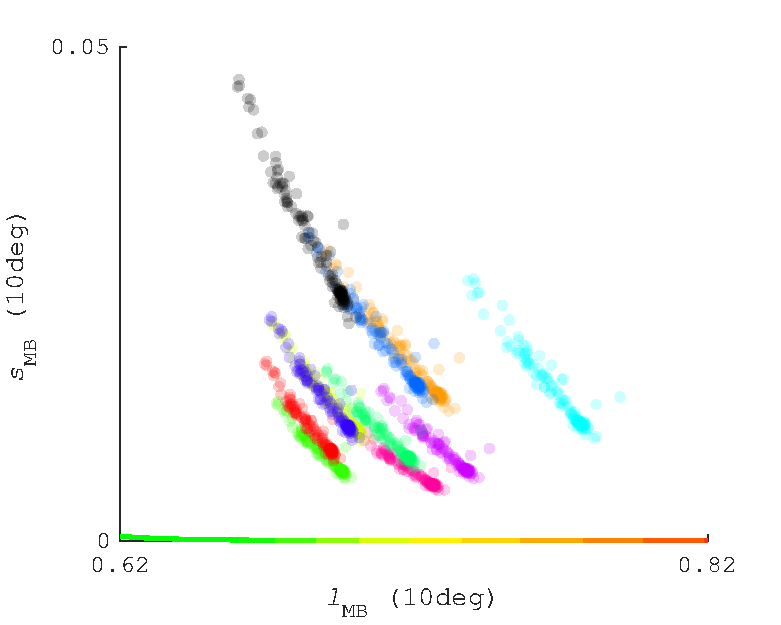
\includegraphics[max width=\textwidth]{figs/comp/predictingChromaticity/BasicMB_2.pdf}
    \caption{\gls{MB} chromaticities of 130 daylight illuminants (black points), and for 10 reflectances under each illuminant (coloured points). Colours not linked to real colours, solely used to distinguish different surafaces from one another). The edge of the spectral locus is visible along the lower edge.}
    \label{fig:MB}
\end{figure} 

% -------------------------- %

\section{Recovering the chromaticity of daylight}

The simplest computational method to achieve rough colour constancy is through normalisation of input signals by the hypothetical input signals to the illuminant. It is the implicit assumption in previous experiments that a melanopic signal could act as a cue to the chromaticity of the illuminant.

This is what \citet{maloney_physics-based_2001} refers to as the `RGB heuristic'. In most situations appearance of a scene under two different illuminants will be relatable via the chromaticity of those illuminants.\footnote{However, it should be noted that there is no mathematical reason for this to be strictly true due to different colour rendering properties.}

\bigskip
\noindent
Initially, two questions were proposed:
\begin{enumerate}
\item Considering only daylight spectra (excluding reflective surfaces), can a melanopic signal predict the chromaticity of daylight? \item Now considering also object reflectances, can a melanopic signal predict the chromaticity of the daylight? 
\end{enumerate}

\subsection{First level signals}

In this chapter the terminology of \citet{barrionuevo_contributions_2014} shall be employed; following their usage `first level signals' are those which are direct photoreceptor catches (or analogues, such as $XYZ$ tristimulus values), and `second level signals' are those computed by comparison of one signal and one or more other signals (such as $xy$ or \gls{MB} chromaticity values).

In order to visualise the relationship between the chromaticity of the illuminant and the resulting receptor catches, three-dimensional plots were made displaying $l_{\text{MB}}$ against $s_{\text{MB}}$ against $[L,M,S,I]$ in turn. \gls{MB} chromaticity space was chosen due to its status as a physiologically based chromaticity diagram, following the logic that if biologically plausible mechanisms are sought, then computations in a space best representing the real space are preferable. The plot for $I$ is shown in Figure \ref{fig:level1}. Other plots closely resembled this one. It can be seen that although there exists some relationship between the chromaticity values of the illuminants and the $I$ values, it does not appear as though one could be used to reliably predict the other. 

There is an almost bimodal relationship; all that can be gained from this relationship is the understanding that if the $I$ value is above a certain threshold, it is likely to be in a group with a relatively low $s_{\text{MB}}$ and relatively high $l_{\text{MB}}$ value. The real-world correlate of this is - \textit{if the daylight is bright enough, I can be fairly confident that the chromaticity of light will be relatively warm in colour.} This is as expected, since the brightest daylight conditions are likely to be those with unobstructed direct sunlight, which is warmer in \gls{CCT} than illumination provided by the blue sky. This relationship could not be used to predict the precise chromaticity of an illuminant. A near-identical trend is seen when surfaces are considered (the coloured points in Figure \ref{fig:level1}).

\begin{figure}[htbp]
    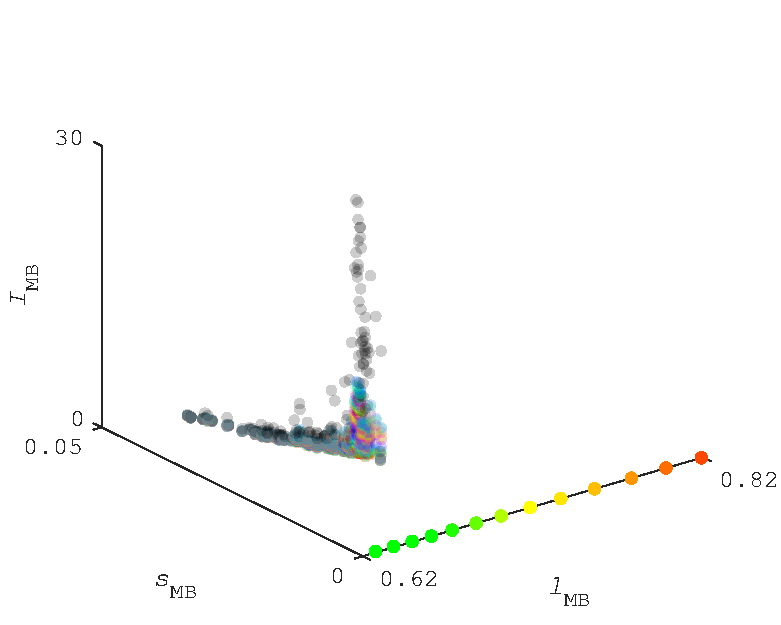
\includegraphics[max width=\textwidth]{figs/comp/predictingChromaticity/CvsI.pdf}
    \caption{\gls{MB} chromaticity of 130 illuminants plotting against the $I$ values for the illuminants alone (black points) and 10 different surfaces (coloured points). The edge of the spectral locus is visible along the $l_{\text{MB}}$ edge of the diagram.}
    \label{fig:level1}
\end{figure} 

\subsection{Second level signals}
Following this, similar plots were made which plotted $l_{\text{MB}}$ against $s_{\text{MB}}$ as before, but now plotted the various second level combinations of $[L,M,S,I]$, created by considering one signal divided by another (e.g. $L/M$), on the z-axis. These plots are shown in Figure \ref{fig:allComboSignals}. The plots created all showed clear and relatively simple relationships between chromaticity and these new derived signals, at least for the illuminant-only values. 

\begin{fullpagefigure}
\figpdf[pages=-,rotate=90, offset=75 -75]{figs/comp/predictingChromaticity/allComboSignals.pdf}
\caption{Relationship between chromaticity and second level signals. Plotted on the x-axis here is $l_{\text{MB}}$, with second level signals on the apparent y-axis. During analysis these plots were three dimensional, with the apparent y-axis being a z-axis and the x-axis joined by a y-axis of $s_{\text{MB}}$. As before, black points indicate direct illuminant values, with coloured values corresponding to surface reflectances (though the colours do not relate the surfaces other than to distinguish one from another). It can be seen that on a per object basis (incl. no object) there is good correlation between chromaticity and all of the above signals. A similar relationship holds for the $s_{\text{MB}}$ perspective.}
% See gifs online at...
\label{fig:allComboSignals}
\end{fullpagefigure}

A similar trend was seen for each individual surface as was seen for illuminant-only, however these relationships appear to be offset from that for a perfect reflector.

\subsection{A PCA interpretation}

These results seem to make intuitive sense based if we consider the daylight dataset from a principal components perspective. For this dataset \gls{PC1} is broad and relatively smooth, and accounts for 99.952\% of the variance, and so a first level signal in any part of the spectrum is going to essentially track this component. 

\begin{figure}[htbp]
 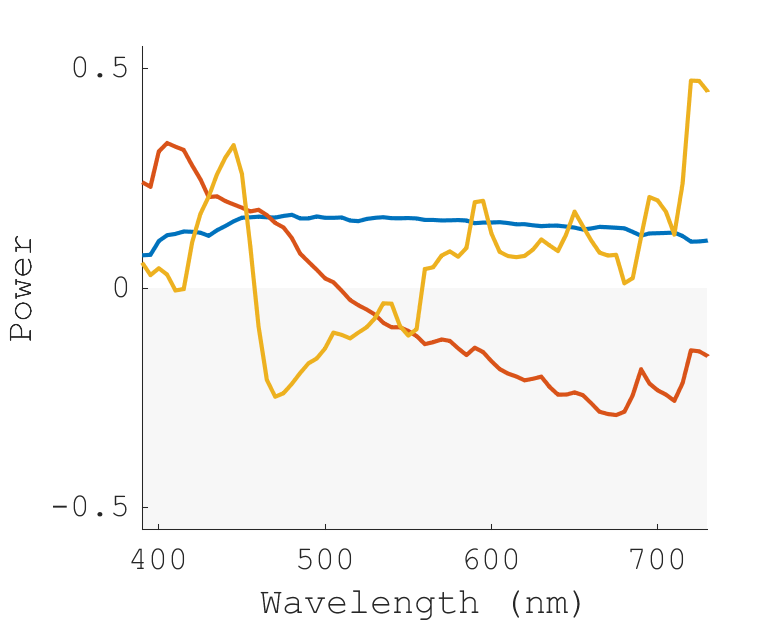
\includegraphics[max width=\textwidth]{figs/comp/melcomp_3/8.png} %legend required
 \caption{The first 3 principal components for the Granada daylight dataset, after weighting to prioritise the visible spectrum. PC1 is in blue, PC2 in red and PC3 in yellow. These first three components account for 99.952\%, 0.037\% and 0.005\% of variance respectively.}
 \label{fig:PCA}
\end{figure} 

\Gls{PC2} is relatively smooth and monotonic (and accounts for 0.037\% of the variance). Almost any comparison between signals at different points in the spectrum (second level signal) is going to roughly track this component (though the relative contribution of this component will slightly depend on the value of \gls{PC1}).

% Could add a plot relating chromaticity to PC2 and PC3 here.

Each surface meanwhile, will differentially reflect different parts of the spectrum, meaning that this sampling of \gls{PC2} will vary from surface to surface, but the same overall trend will be followed.

%\begin{figure}[htbp]
%  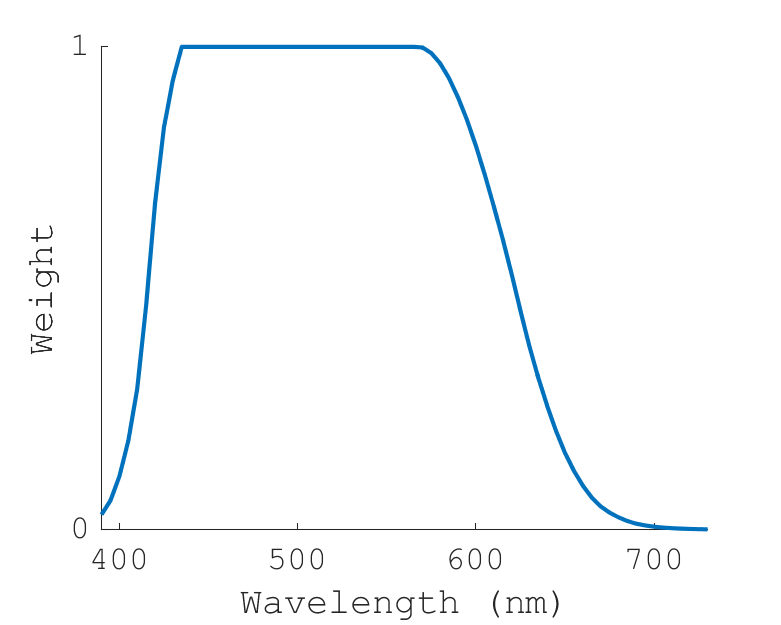
\includegraphics[max width=\textwidth]{figs/comp/melcomp_3/vw.png}
%  \caption{The variable weightings applied during the \gls{PCA} analysis. Generated by tracing the upward ramp of the S-cone sensitivity being used, plateauing at unity until the decrease of the L-cone sensitivity, and then following the decrease of the L-cone sensitivity.}
%  \label{fig:VW}
% \end{figure} 

\subsection{Relationships as artefacts}

For many of these signals however, such relationships are to be expected\footnote{My thanks go to Manuel Spitschan for convincing me of this point.}. For example, a relationship between $l_{\text{MB}}$ and $L/M$ should be expected, since $l_{\text{MB}}$ is defined as the sum of weighted components of $L$ and $M$. To confirm this, a control condition was performed, where $[L,M,S,I]$ was replaced by randomly generated values, and the second level signals were generated as before. The results can be seen in Figure \ref{fig:allComboSignals_rand}. Relationships between secondary signals derived from $L$, $M$ or $S$ signals still showed correlations with chromaticity (albeit now points fell on a plane, instead of a line), whereas signals with a $I$ component showed only minimal coherence, forming a noisy cloud in three-dimensional space. This implies that should the melanopic signals correlate with chromaticity, that this is not simply a computational artefact of the way in which chromaticity is calculated.

\begin{fullpagefigure}
\figpdf[pages=-,rotate=90, offset=75 -75]{figs/comp/predictingChromaticity/allComboSignals_rand.pdf}
\figpageside{}
\caption{As per \ref{fig:allComboSignals} but where $[L,M,S,I]$ was replaced by randomly generated values, and the second level signals were generated from these instead of real values. Blue is used to distinguish this random data from previous real data. Note that different rotations have been applied to some of the subplots to best display the correlations.}
\label{fig:allComboSignals_rand}
\end{fullpagefigure}

This example shows that if a melanopic signal exhibits correlation with a chromatic signal \emph{not} due to the underlying mathematics of how chromaticity is calculated, and that any relationship must follow from a genuine regularity in the data.

\bigskip
\noindent
To summarise this section:

\begin{enumerate}
   \item A basic melanopic signal, computed from direct daylight measurements, cannot predict chromaticity, other than a crude estimation of whether a measurement is direct sunlight or not. \emph{Figure \ref{fig:level1}}
    \item The same can be said for melanopic values computed for daylight reflected off a surface. \emph{Figure \ref{fig:level1}}
  %  \item A first level melanopic value is highly correlated with first level cone signals. \emph{Figure \ref{fig:tristimCorrelation}}
    \item There are relatively strong and simple relationships between hypothetical second level signals and illuminant chromaticity. \emph{Figure \ref{fig:allComboSignals}}
    \item When considering surfaces, these relationships are maintained, but offset differently for each surface. \emph{Figure \ref{fig:allComboSignals}}
    \item Some of these correlations appear to be nothing more than computational artefacts (\emph{Figure \ref{fig:allComboSignals_rand}}). Notably, the melanopic second level signals did not seem to be such artefacts.
\end{enumerate}

\clearpage


% -----------------------------------------%
\section{Transformation to an illuminant-independent space}

Whilst estimating the chromaticity of the illuminant is one way in which colour constancy might be achieved, it is also possible that some transformation might exist which delivers signals into an illuminant-independent space but which doesn't explicitly depend upon an estimate of the chromaticity of the illuminant.

Considering that the absolute melanopic values seemed to offer little predictive benefit (see Figure \ref{fig:level1}) the choice was made to create a normalised melanopic value similar in nature to the MB values. Following Equation \ref{eq:MB}, but with a melanopic value in place of the $S$ value, allowed for the creation of what shall be termed the $i_{\text{MB}}$ values.

\subsection{A melanopic signal as a third dimension}

In order to try to better understand the relationships between the \gls{MB} chromaticities and the new $i_{\text{MB}}$ values, and to understand what types of corrective computations might be effective, consideration was given to the $i_{\text{MB}}$ signal as a third dimension upon the already two-dimensional \gls{MB} chromaticity space, such as shown in figure \ref{fig:ZL}. This allowed the consideration what properties a signal upon this third dimension would need to provide to the overall three-dimensional point cloud in order for a transformation to occur which would transform the values into a two-dimensional illuminant-independent space.

\begin{figure}[htbp]
 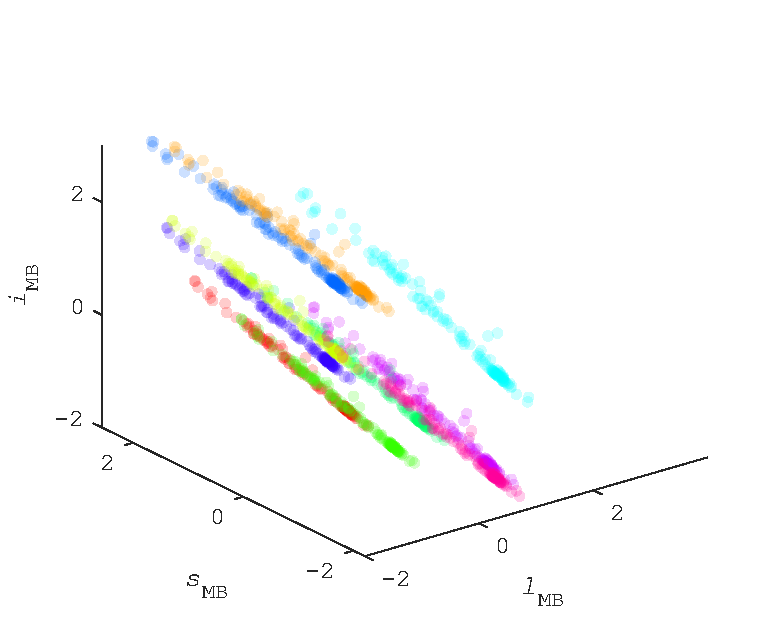
\includegraphics[max width=\textwidth]{figs/comp/thirdDimension/ZL.pdf}
 \caption{X and Y axes are a \gls{MB} chromaticity space, and the Z axis is $i_{\text{MB}}$. Data plotted are same as previous section.}
 \label{fig:ZL}
\end{figure}

It was found that a log transform applied to the $[lsi]_{\text{MB}}$ data made relationships between the various signals more linear, and the data much more normally distributed. The data were also zero-meaned and normalised for standard deviation so that the signals were on like scales.

A range of speculative transformations were performed, to demonstrate the types of transformation that could be used to transform colour signals to illuminant-independent colour signals. A rotational transformation was successful (analogous to changing the perspective as in figure \ref{fig:viewpoint}) and additionally a weighted additive model was found to be rather successful. No satisfactory model was found where a purely multiplicative transformation was applied.

Thinking about a corrective signal as an additional dimension upon a \gls{MB} chromaticity space allows for consideration of requisite or desirable properties that this third signal should imbue upon the three-dimensional cloud of points. I have identified one requisite property, and one desirable property. 

The requisite property for such a signal, as already suggested, is that it should differ from other chromatic signals enough to allow for the point cloud of chromatic points to be significantly \emph{non-planar}. This in turn allows for a projection upon two-dimensional space which has the potential to be illuminant-invariant.

The desirable property is that it should be \emph{roughly monotonic} with respect to other chromatic signals. This allows a one-to-one mapping of colour signals to illuminant-independent colour signals, where a non-monotonic relationship does not necessarily do so. This is not a strict requirement, since the corrective function only needs to be one directional, but non-monotonicity would exclude simple transforms (such as linear additive or rotational).

Another key finding at this stage was that there is a perspective upon a three-dimensional point cloud ($[l_{\text{MB}},s_{\text{MB}},i_{\text{MB}}]$) from which points from like objects clustered well, such as in figure \ref{fig:viewpoint}. This property shows that there is at least one transformation such that the points could be projected upon a two-dimensional plane where the illuminant-dependence was greatly reduced whilst the inter-object chromatic relationships were retained. 

\begin{figure}[htbp] % redo this. Is this log data?
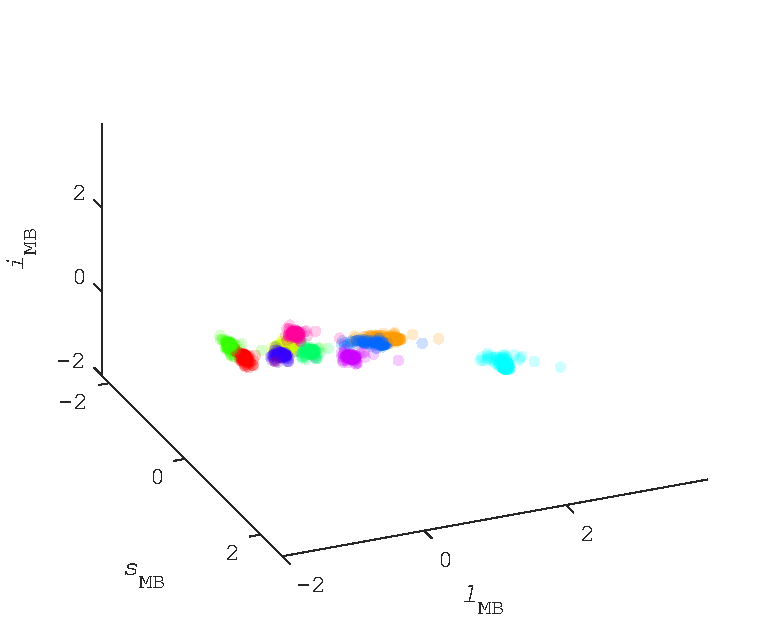
\includegraphics[max width=\textwidth]{figs/comp/thirdDimension/viewpoint.pdf}
 \caption{Figure \ref{fig:ZL} rotated to a perspective where it can be seen that the points project upon a two-dimensional plane in a clustered fashion whilst not degrading to a line within that space.}
 \label{fig:viewpoint}
\end{figure} 

Note that such a perspective would not be possible for a space where the third dimension were a near-duplicate of the first or second, since in this case all points would lie upon a plane. This would be the case in circumstances where a corrective signal too closely resembled the visual signals. The fact that points do not lie on a plane shows that there is some decorrelation between $i_{\text{MB}}$ and both $l_{\text{MB}}$ and $s_{\text{MB}}$. The fact that they do not lie on a plane and instead diverge from this plane in a surface-dependent fashion (as opposed to noisily diverging) suggests that the $i_{\text{MB}}$ may present a means to separate the contribution from illuminant and surface. 

% \subsection{Measuring planarity}

% It also introduced a measure of non-planarity, calculated by performing a principal components analysis on the cloud of points $[l,s,i]_{\text{MB}}$, and looking at how much variance was unaccounted for by the first two principal components. It was found that there were two parts of the spectrum where an effective corrective signal (in terms of non-planarity); firstly at around and just higher than the peak spectral sensitivity of melanopsin, and secondly with a melanopsin shift of about positive 75nm (see `Standard' in Figure \ref{fig:PC3}). It was found that minor changes in parameters used to make these calculations, such as surface set used or observer used, could have moderate effects on the optimal sensitivity for a sensor whose task was to provide a signal for transforming cone signals (see others in Figure \ref{fig:PC3}).

% \begin{figure}[htbp]
%     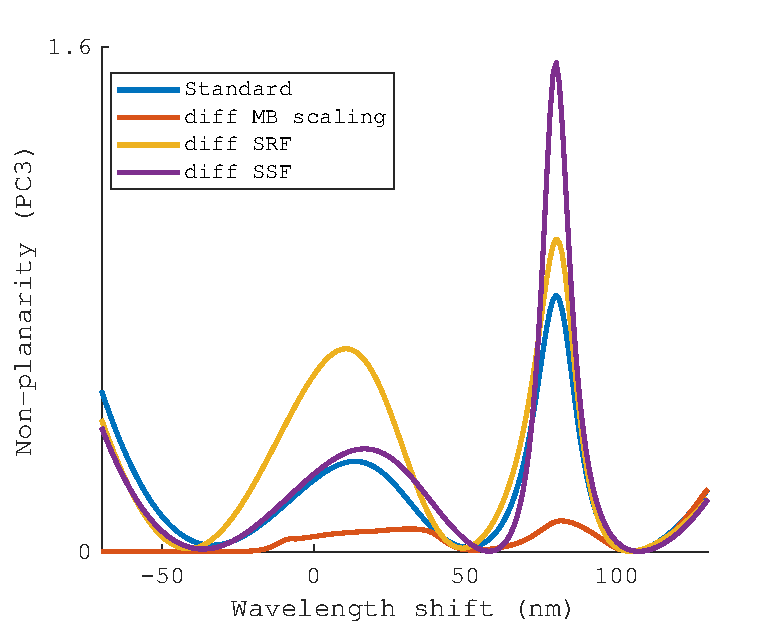
\includegraphics[max width=\textwidth]{figs/comp/melcomp_6/PC3.pdf}
%     \caption{}
%     \label{fig:PC3}
% \end{figure} 



\subsection{Additive/Subtractive model}

It was found through an optimisation procedure that through addition or subtraction of weighted $i_{\text{MB}}$ values, as per equation \ref{eq:correction} a conversion to an approximately illuminant-independent could be performed. The optimisation initially sought optimal weights for the scaling factors with the goal of minimising the overall spread of chromaticities (measured as standard deviation of the entire set)\footnote{This was later amended to the intra-group spread of chromaticities, measured as standard deviation of within each group. This had a relatively minor impact, $k_{1}$ = 0.57, and $k_{2}$ = -0.94.}. The results of applying Equation \ref{eq:correction} can be seen in figure \ref{fig:corrected}. %The effect of different weights can be seen in Figure \ref{fig:minSD}. 
It can be seen that the points now roughly cluster together by object, with less smearing induced by changes in illuminant (compared to Figure \ref{fig:MB}).


\begin{subequations} \label{eq:correction}
\begin{align}
l_{\text{MB}}* &= l_{\text{MB}} + k_{1}i_{\text{MB}}\\ %these will have changed
s_{\text{MB}}* &= s_{\text{MB}} + k_{2}i_{\text{MB}}
\end{align}
\end{subequations}

where $k_{1}$ = 0.44, and $k_{2}$ = -0.91.

\begin{figure}[htbp]
    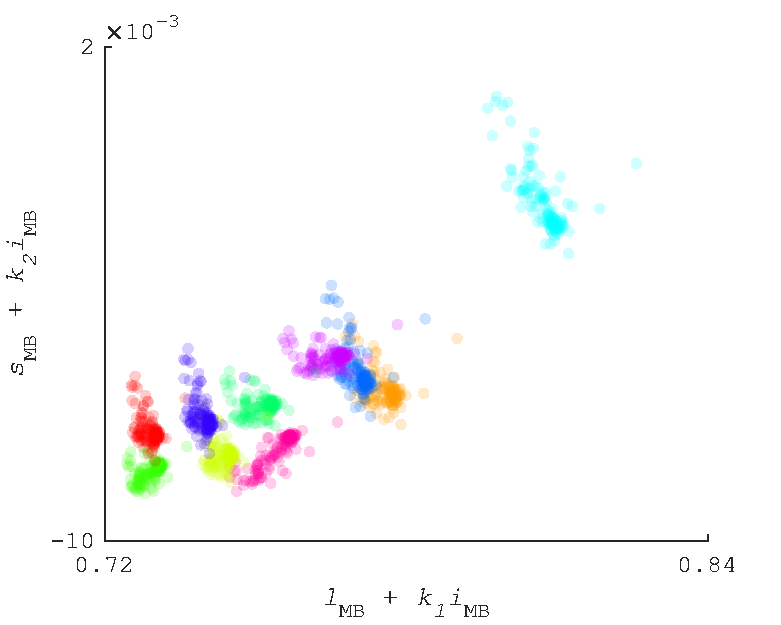
\includegraphics[max width=\textwidth]{figs/comp/transformToIllIndSpace/correctedChromaticities.pdf}
    \caption{\gls{MB} chromaticities for 10 reflectances under 130 daylight illuminants, corrected by the corresponding $i_{\text{MB}}$ value as per Equation \ref{eq:correction}.}
    \label{fig:corrected}
\end{figure} 

% \begin{figure}[htbp]
%     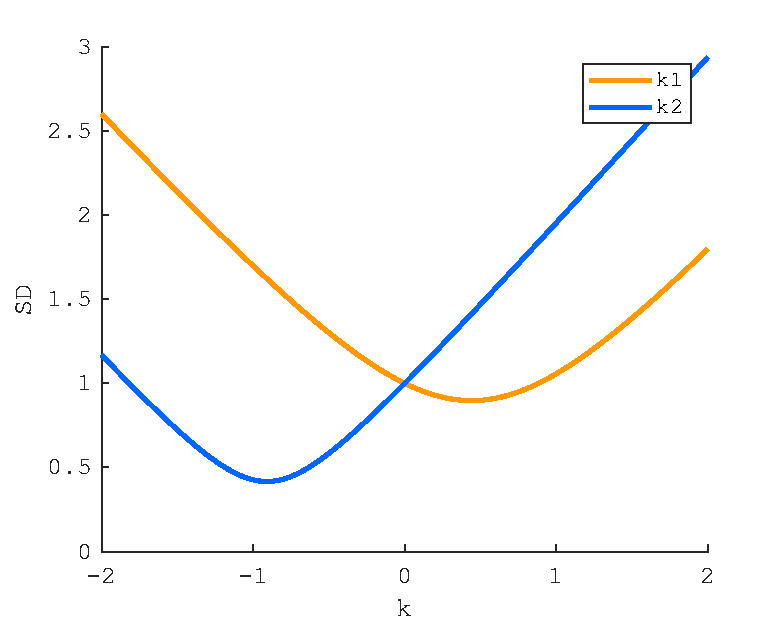
\includegraphics[max width=\textwidth]{figs/comp/transformToIllIndSpace/kvsSD.pdf}
%     \caption{The effect on whole-set SD of differently weighted additions/subtractions of the $i_{\text{MB}}$ values. The minima of these functions are taken as the values for $k_{1}$ and $k_{2}$.}
%     \label{fig:minSD}
% \end{figure} 

It was unclear however whether this advantage would be gained by the addition of any new signal, or whether the melanopsin signal was in any way optimal. With this in mind, the peak spectral sensitivity of the melanopsin function was parameterized, to consider whether shifting the sensitivity of the melanopsin function along the wavelength spectrum affected the performance of such a signal. Each new sensitivity function was allowed the benefit of its own weighting optimisation, allowing different scaling factor weights. The results of this computation can be seen in figure \ref{fig:opt}. 

\begin{figure}[htbp]
    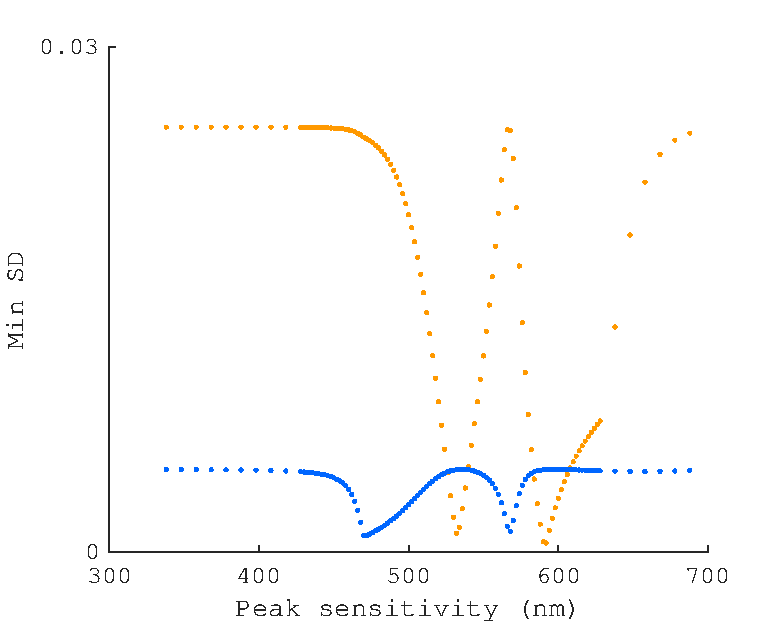
\includegraphics[max width=\textwidth]{figs/comp/transformToIllIndSpace/offsetrange1.pdf}
    \caption{The results of an optimization where the spectral sensitivity of the nominal melanopsin fundamental was shifted along the spectrum. Generated using melcomp\_1\_caller.m for iteration.}
    \label{fig:opt}
\end{figure} 

It can be seen that standard deviation minima for $l_{\text{MB}}$* occur at 532nm and 590nm, and for $s_{\text{MB}}$* at 444nm and 568nm. This would suggest that the optimal spectral sensitivity for a receptor employed to correct the signals from the various cones would be at these points in the spectrum. However, if we plot the transformed chromaticities computed using hypothetical signals at these wavelengths, we see that the results are not an obvious improvement. In Figure \ref{fig:590} the results of using a nominal melanopic signal with a peak spectral sensitivity of 590nm are shown. Group SD is low, but different surfaces are not particularly well distinguished from each other. We witness good colour constancy, at the expense of chromatic discrimination\footnote{At my poster at VSS David Brainard referred to this as the `Ford Model of Colour Constancy' - you can have any colour, so long as it's black.}. This is obviously not ideal.

\begin{figure}[htbp]
    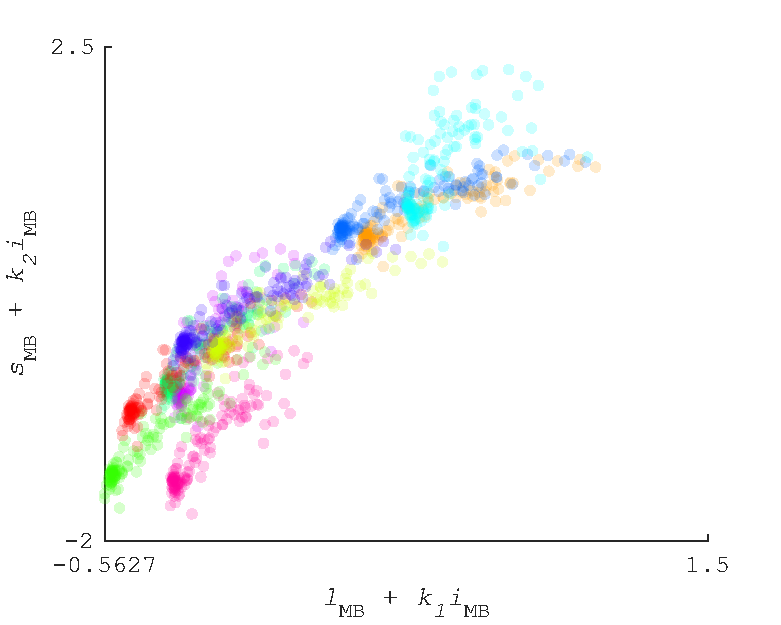
\includegraphics[max width=\textwidth]{figs/comp/transformToIllIndSpace/correctedChromaticities_range590.pdf}
    \caption{The `corrected' values using a nominal melanopic signal with a peak spectral sensitivity of 590nm.}
    \label{fig:590}
\end{figure} 

This result made it very clear that more though was required regarding how `success' was calculated.

The actual desired behaviour would be to minimise internal variance for each reflectance group (rather than the whole set), whilst maintaining at least some distinction between inter-reflectance groups. There are various ways to implement this, which shall be covered in the following sections. %

\bigskip
\noindent
To summarise this section:
\begin{enumerate}
    \item Following earlier findings that a second level signal seemed more likely to show a relationship to chromaticity, and be likely to sample the \gls{PC2} values of daylight, hypothetical $i_{\text{MB}}$ values were computed.
    \item An extended range of transformations were trialled: additive/subtractive, rotational and multiplicative. All but multiplicative showed promise.
    \item One requisite and one desirable property for a hypothetical third signal were identified: decorrelation (leading to non-planarity) and monotonicity. 
    \item A perspective upon the three-dimensional $[lsi]_{\text{MB}}$ space was found where points diverged from a plane in a surface-dependent fashion. \emph{Figure \ref{fig:viewpoint}}
    \item A basic additive/subtractive algorithm was applied, which seemed to reduce the spread of chromaticities in a meaningful fashion. \emph{Figure \ref{fig:corrected}} 
    \item It was found that when the melanopic value was replaced by signals generated from different spectral sensitivities, some hypothetical signals appeared to be more successful than a melanopic value. These signals performed very well by the metric of whole-set standard deviation, but in practice would make very poor corrective signals due to the reduced discriminability between surfaces. \emph{Figure \ref{fig:590}}
\end{enumerate}

\clearpage




% -----------------------------------%
\section{Assessment of colour constancy algorithms}

The basic mechanism of an additive/subtractive model of melanopic colour constancy seems worthy of further scrutiny. However, we have seen that care is required in defining what is considered successful performance for a colour constancy algorithm. Broadly speaking, we would like our algorithm to be judged on its ability to allow for \emph{recognition} (reliably remapping points from a specific surface to a specific point in appearance space) and \emph{discrimination} (creating distinct representations of different surfaces)\footnote{The ideal colour constancy algorithm would distinguish between all spectrally distinct surfaces, no matter how minor their distinctions. However, here we are more interested in uncovering a mechanism which may be used by the human visual system, and so it seems sensible to limit the requirement to separation of surfaces which would generally be seen as chromatically distinct.}.

Different schools of thought within colour constancy research have used different methods for assessing proposed algorithms, mirroring subtle differences in their respective conceptual goals. Three subtle variants can be described via representative research questions:

\begin{itemize}
\item{How do humans achieve colour constancy?}
\item{How do we predict what humans perceive?}
\item{How can we colour correct digital photos to best emulate the original appearance of the scene to the photographer?}
\end{itemize}

The first group have tended to assess their proposed solutions in the context of biological and physical plausibility. Where solutions in this group rely upon some regularity in the environment, discussions gravitate to the value, ubiquity, and veracity/validity of this regularity (see Hurlbert's table \cite[p.~295]{hurlbert_computational_1998} which sorts a range of colour constancy algorithms by the assumptions that they rely upon). Alternatively, studies can remove the cue or cues under investigation from a controlled visual scene and in some way measure the impact upon an observer's state of chromatic adaptation \cite{kraft_mechanisms_1999}. I am not aware of a standard measure for quantifying the ability or biological plausibility of a particular proposed algorithm.

The second group have made considerable progress in the development of the \Glspl{CAT} which are used within \Glspl{CAM}, through the collection of corresponding colour datasets (pairs of colorimetric values where the the first member of each pair under a first illuminant matches in appearance the second under a second illuminant). Models are then fit to these datasets such that the appearance of an arbitrary colour under the one illuminant could be predicted under the other, and vice versa. The effectiveness of a model is quantified by considering how well the model fits data which was independently collected \cite{cie_cie_2004-1}.

The third group focuses on estimating the tristimulus values or colorimetry of an unknown illuminant from the pixels of a digital photographic image. There is obvious crossover between this group and the previous groups, for two reasons.
Firstly, the human visual system could compute relatively meaningful estimates of surface reflectance properties if the illumination spectra could be estimated with moderate accuracy \cite{maloney_computational_1984}. Secondly, where the goal is to output an image which appears as it would to a human observer, there is implicitly a goal to understand how an observer might be performing this computation. This group traditionally quantifies success of algorithms by how well they can compute an illuminant estimate in terms of its RGB values in a camera-specific colour space.

There is no clear fit between existing models of assessment and the specific goals of the algorithm under assessment. The most natural fit is within the first group, since the key interest is in whether a melanopsin-based signal provides a valuable tool to a biological system in solving an ecological problem (and thus whether it might be sensible for it to be in use in real biological systems). However, it is unclear at this stage what the mechanism by which such a system may operate is, and so the discussion of what assumptions such a mechanism may rely on seem overly abstract at this stage.

Of clearer applicability is the work of Barnard et al. \cite{barnard_comparison_2002} (later used by \citet{hordley_reevaluation_2006} and \citet{gijsenij_computational_2011}). They propose a method whereby spectral measurements of illuminants and surfaces are used to create `synthesized' data, representing each surface under each illuminant, which can be used as an input to a colour constancy algorithm. Since the ground truth is known here, the results can be quantitively assessed. 

There are some amendments to their process which are required if we are to use it here. Firstly, the data used in their experiments comprises natural and non-natural surface reflectances and illuminants, which is suitable for their purposes of assessing algorithms designed for digital cameras, but is unsuitable here for assessing an algorithm to understand its ability in a natural environment (the environment which would have influenced the natural evolution of biological systems). Therefore, the reflectance and illuminant data will need to be limited to naturally feasible data. Secondly, their performance metrics again relate to their problem rather than ours: they consider only the accuracy of the estimated white point, and whilst this may be useful to a biological system, the grander goal is a conversion of chromaticities to an illuminant-independent surface appearance space. An illuminant estimate is one way to reach this goal, but it is not fundamentally necessary, and the accuracy of this value does not necessarily provide a good measure of effectiveness of the whole system.

One performance metric which more closely matches the goals of this study is that provided by Forsyth \cite[p.~19]{forsyth_novel_1990}, who suggests the ``the median Euclidean distance of the outputs from the average (over the different lights) output, for each chip. This median is then normalised by the Euclidean magnitude of the outputs.'' This value provides an insight into the nature of clustering of points following a transform, which can be considered as loosely related to our fundamental goal of allowing for recognition (a point being mapped to roughly the point it should be). However, no regard is given to our second fundamental goal of discrimination. Indeed, an algorithm which outputs two clusters of points which lay directly atop each other, even if these clusters represented vastly different objects, would be rated as successful, if these clusters were particularly tightly clustered.

% ---------------------------------- %
\subsection{K-means clustering as an assessment tool}

Whilst the clustering metric of Forsyth is a step in the right direction, it doesn't quantify disriminability, and there is no clear way in which it could be amended to do so. Further, it would be preferable to consider these two characteristics in unison since they are valuable only in relation to eachother: we could allow for loose clustering is the cluster centres were distant, but would require tight clusters if they were close. 

To address this shortcoming I propose the following: that the output of an algorithm (where the input is a batch of synthetic data such as in the method of \citet{barnard_comparison_2002}) should be subjected to a k-means clustering (this is easy where synthesised data is used and $k$ is known) and this output in turn should be marked against the known groupings of the original input data. This marking would reveal how well the algorithm had remapped points into clusters relating to their original grouping, and how seperable the clusters are. A suitable number of repetitions of the k-means clustering is advisable, to avoid local minima. 

% A more extensive framework of testing a melanopic correction against other colour constancy algorithms was introduced, following the framework of \citet{barnard_comparison_2002} (later used by \citet{hordley_reevaluation_2006} and \citet{gijsenij_computational_2011}) A \gls{GW}, a \gls{BiW}, and a \gls{DN} algorithm were used as benchmarks.

To test/demonstrate such a procedure, let us consider the plots from Figure \ref{fig:corrected} and \ref{fig:590}. Whilst the simple measure of whole-set standard deviation reports the latter as the more successful output, the k-means-mark for these outputs is 0.8915 and 0.5662 respectively, which tallies with our intuition of which instance of the algorithm has performed better. The K-means selections for each are visualised in Figures \ref{fig:KM1} and \ref{fig:KM2}.

Before the k-means clustering algorithm was applied, data were again zero-meaned (no effect on algorithm, only neatens later presentation) and normalised by standard deviation (medium/large effect on algorithm, resulting in equal weights given to variance in either dimension of \gls{MB} space).

\begin{figure}[htbp]
 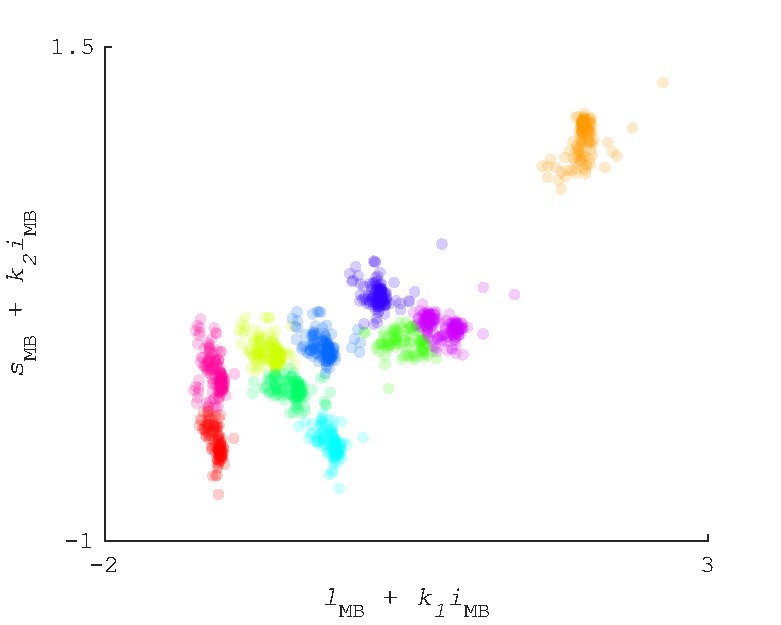
\includegraphics[max width=\textwidth]{figs/comp/KMeansMarkDemo/1.pdf}
 \caption{The data of Figure \ref{fig:corrected}, plotted with colours indicating the groupings chosen by a k-means clustering procedure. Note that the colours do not relate to appearance of surfaces, they are only to indicate groupings. Note also that these colours do not correspond to colours used in the previous figure; the k-means-mark algorithm is not interested in the absolute labelling of groups, rather whether all members from group X have been sorted into group X etc.)}
 \label{fig:KM1}
\end{figure} 

\begin{figure}[htbp]
 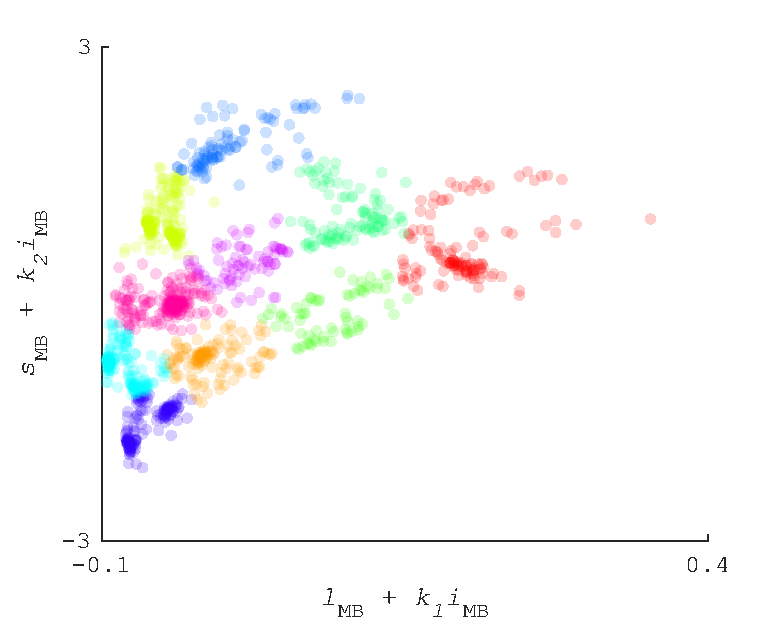
\includegraphics[max width=\textwidth]{figs/comp/KMeansMarkDemo/2.pdf}
 \caption{The data of Figure \ref{fig:590}, plotted with colours indicating the groupings chosen by a k-means clustering procedure.}
 \label{fig:KM2}
\end{figure} 


% ------------------------- %

\subsection{A comparison of four algorithms}

The simple melanopic algorithm (additive/subtractive) was compared with 3 other algorithms: a \gls{GW} algorithm, a \gls{BiW} algorithm and a \gls{DN} algorithm (a baseline condition where no correction was applied).

The structure of \citet{barnard_comparison_2002} was employed, but with the modifications suggested above. %This is shown as a flow diagram in Figure \ref{fig:flow}.

% \begin{fullpagefigure}
% \figpdf[pages=-,rotate=90, offset=75 -75]{figs/comp/flow.png}
% \caption{A flow chart representation of the assessment process.}
% \label{fig:flow}
% \end{fullpagefigure}

% \begin{fullpagefigure}
% \figpdf[pages=-,rotate=90, offset=75 -75]{figs/comp/comparisonFourAlgos/output.pdf}
% \caption{The output of the four algorithms; top left: \gls{DN}, top right: \gls{GW}, botton left: \gls{BiW}, bottom right: \gls{GW}.}
% \label{fig:flow}
% \end{fullpagefigure}


\begin{figure}[htbp]
 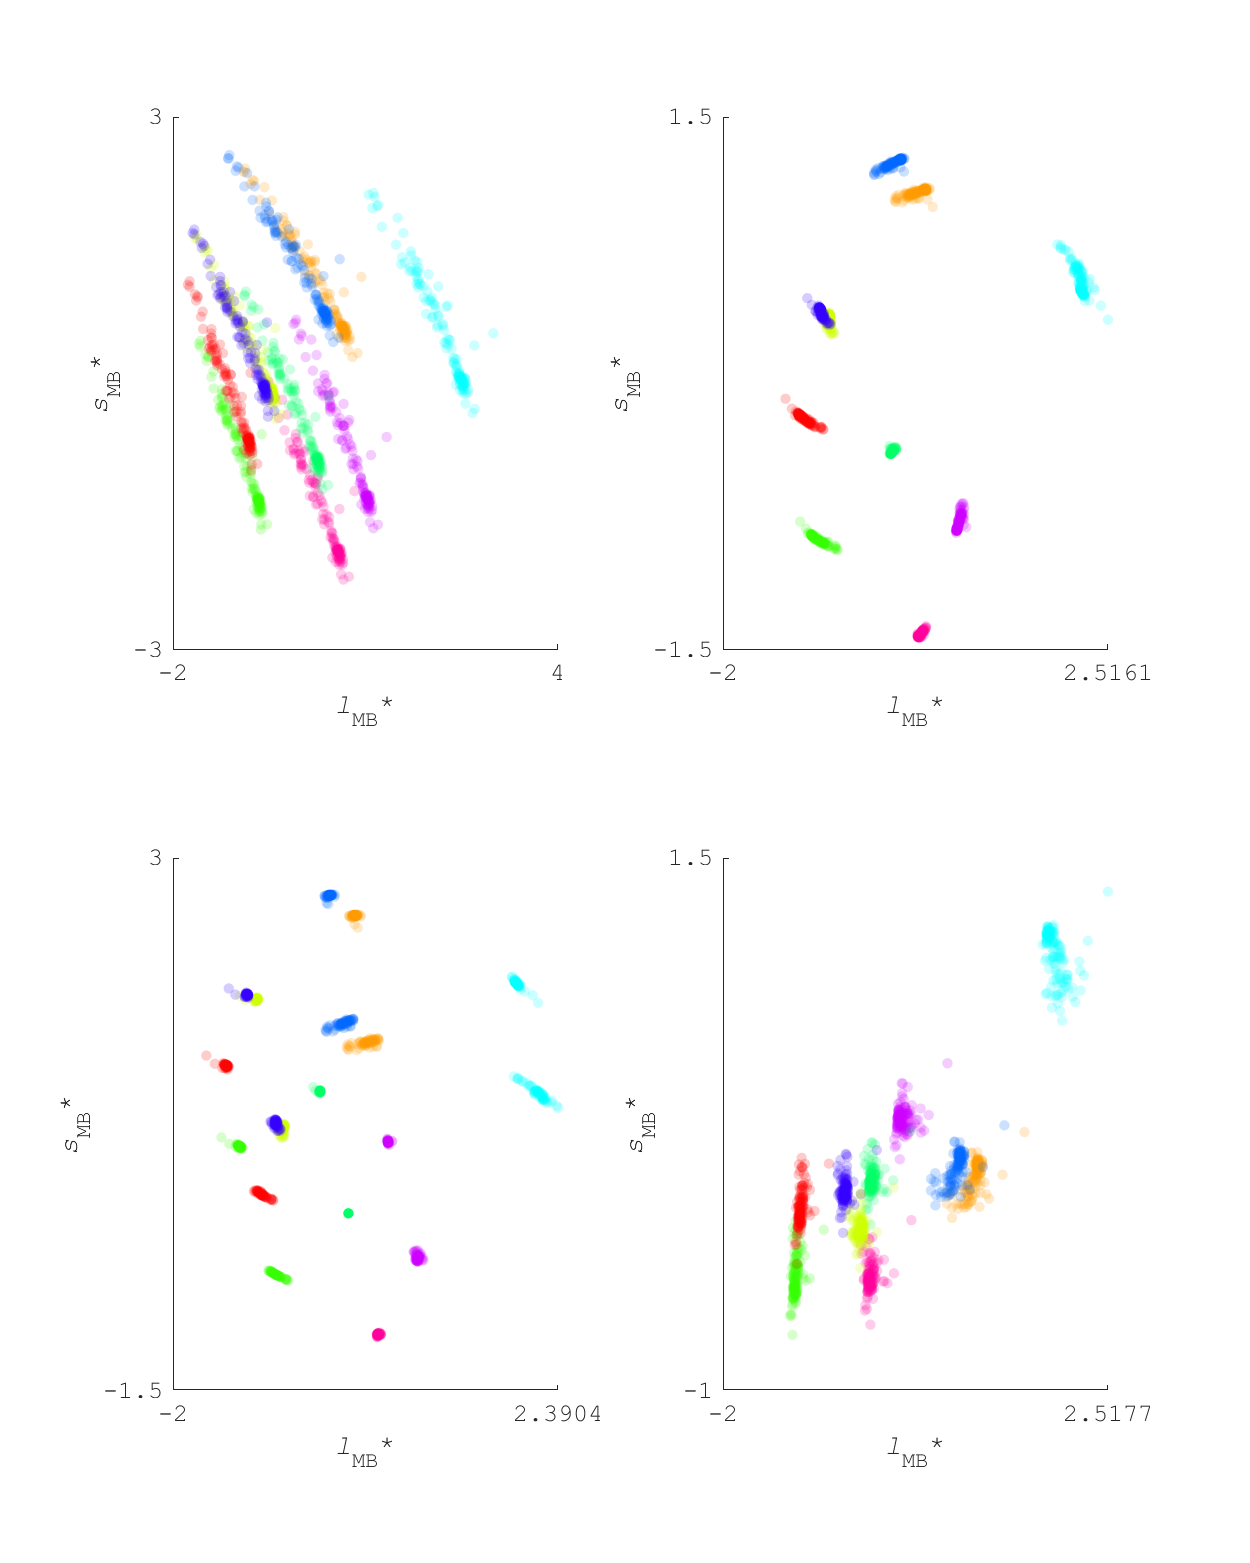
\includegraphics[max width=\textwidth]{figs/comp/comparisonFourAlgos/output.pdf}
 \caption{The output of the four algorithms; top left: \gls{DN}, top right: \gls{GW}, botton left: \gls{BiW}, bottom right: \gls{GW}.}
 \label{fig:4output}
\end{figure} 





% ---------------------------------- %

\subsection{A more naturalistic test case}

\begin{figure}[htbp]
 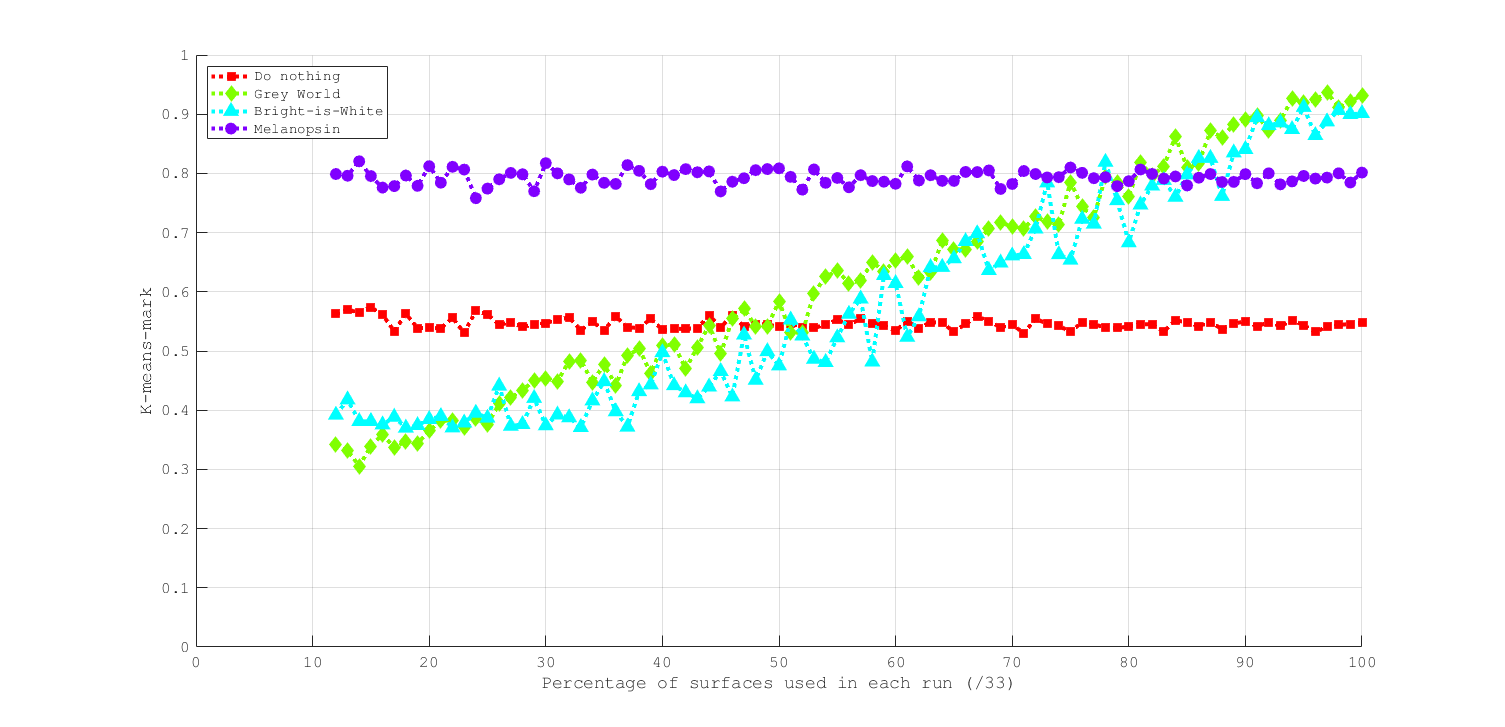
\includegraphics[max width=\textwidth]{figs/comp/melcomp_9/4a_summary.png}
 \caption{The performance of the various algorithms as a function of the available surfaces under any one simulation.}
 \label{fig:4asum}
\end{figure} 

When all surfaces are shown every time, the \gls{GW} and \gls{BiW} algorithms slightly outperform a melanopic transform.


As soon as surfaces start to be randomly removed, performance of \gls{GW} and \gls{BiW} algorithms dropped sharply, whereas the melanopic transform was unaffected. \emph{Figure \ref{fig:4asum}}

% ---------------------------------- %

\section{Optimality of the melanopsin spectral sensitivity}

An additional test, whereby surfaces were randomly removed from a selection was introduced, in order to better parallel the unpredictability of surfaces in natural scenes.

% -------------%

\section{Why is this possible?}

% ------------------------------- %

At this stage the underlying reason for the relative success of these transforms was considered. One potential lead is a curious regularity at the lower wavelengths of the reflectance spectrum of many natural objects. In figure \ref{fig:plateau} it can be seen that there is a plateau in the relative spectral reflectances of some natural objects (a subset of the \citet{vrhel_measurement_1994} reflectances) between roughly 430nm and 480nm, with relatively small deviations within 400nm to 500nm. Another way to visualise this is to calculate the correlation between points on the reflectance function. Such a calculation was performed initially on a combined set of scenes 1-4 of the
\citet{nascimento_statistics_2002}\footnote{Data: \url{https://personalpages.manchester.ac.uk/staff/d.h.foster/Hyperspectral_images_of_natural_scenes_02.html}} hyperspectral reflectance data and
scenes 1-5 of the 
\citet{foster_frequency_2006}\footnote{Data: \url{https://personalpages.manchester.ac.uk/staff/d.h.foster/Hyperspectral_images_of_natural_scenes_04.html}}
hyperspectral reflectance data, and then on three other datasets. See figure \ref{fig:foster} and \ref{fig:others} respectively.

\begin{figure}[htbp]
 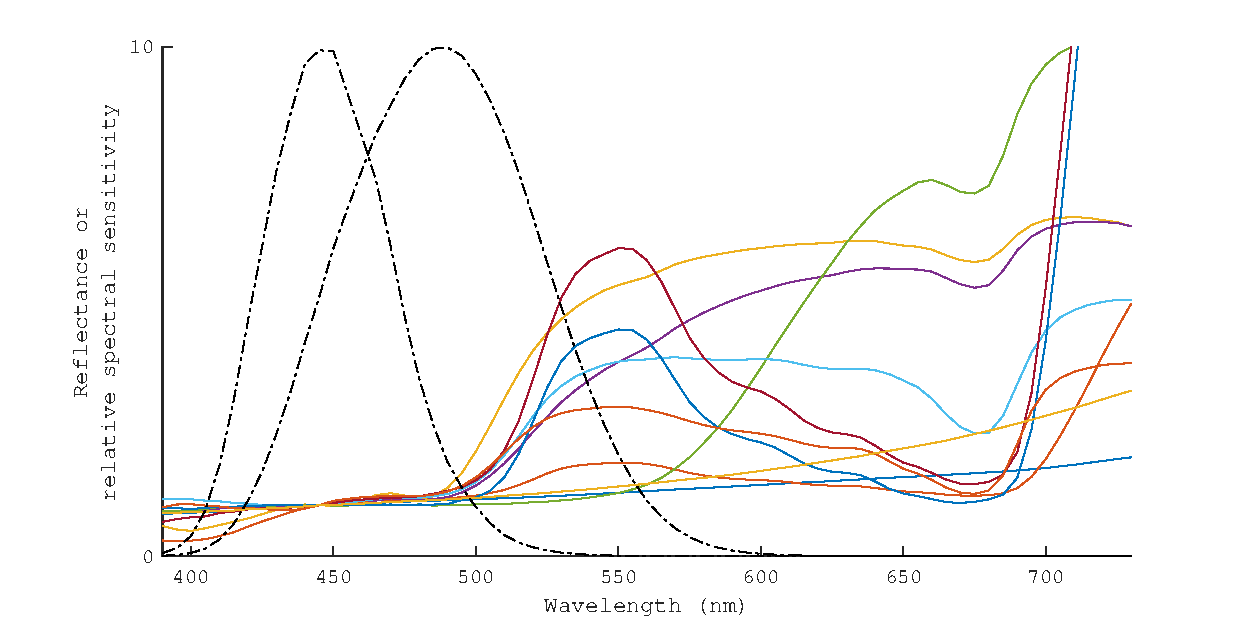
\includegraphics[max width=\textwidth]{figs/comp/melcomp_2_caller/plateau.pdf}
 \caption{The spectral reflectance functions of a subset of the \citet{vrhel_measurement_1994} reflectances (solid lines), normalised at the peak of s-cone sensitivity (CIE 2006 10$^{\circ}$), with the spectral sensitivity of s-cones and melanopsin \citep{lucas_measuring_2014} overlaid (dot-dashed lines).}
 \label{fig:plateau}
\end{figure} 

\begin{figure}[htbp]
 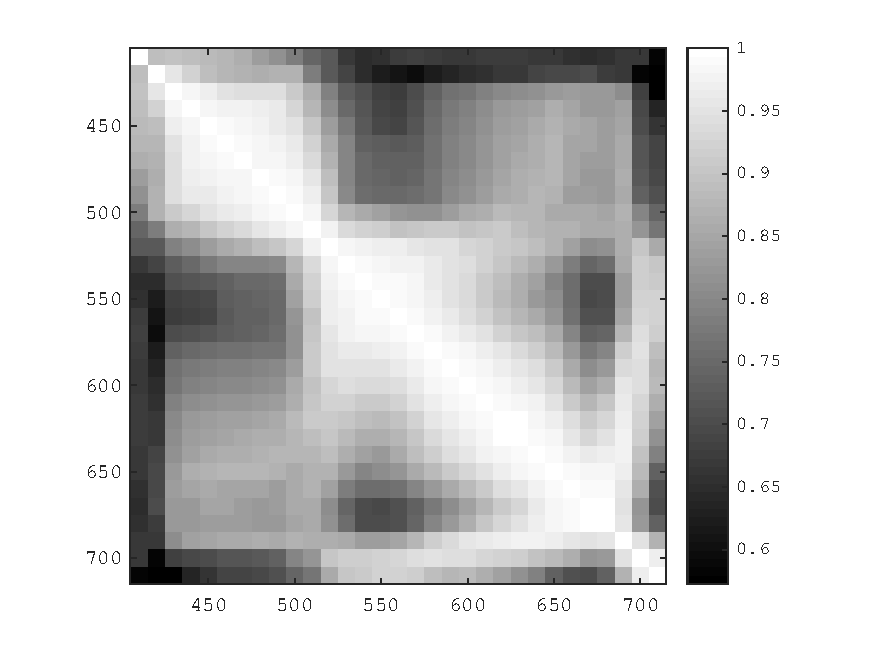
\includegraphics[max width=\textwidth]{figs/comp/nat_cor/foster.pdf}
 \caption{Visualisation of the average correlation matrix for the scenes 1-4 of \citep{nascimento_statistics_2002} and 1-5 of \citep{foster_frequency_2006}. Note the rough square in the top left, indicating an area of increased correlation across different wavelength samplings, and another rough square (though with a faded lower-right corner) in the centre. The dark frame to this figure is likely due to increased measurement noise at these extremes.}
 \label{fig:foster}
\end{figure} %get rid of dotted line on colorbar

\begin{figure}[htbp]
 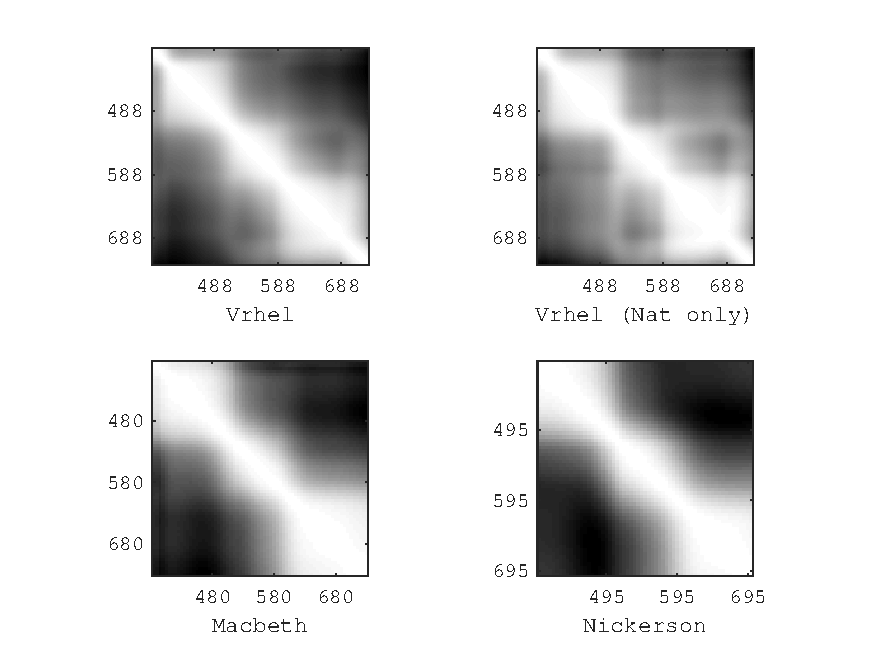
\includegraphics[max width=\textwidth]{figs/comp/nat_cor/others.pdf}
 \caption{As for \ref{fig:foster} but for 3 different sets of data, and one subset. `Vrhel' refers to the object reflectances of \citet{vrhel_measurement_1994} data and `Vrhel (nat only)' refers to a subset of the previous but only using data for surfaces which were deemed `natural'. `Macbeth' refers to measurements of a Macbeth Color Checker. `Nickerson' refers to a set of measurements of Munsell papers (presumably the \citet{kelly_tristimulus_1943} data). Note that whilst we have a selection of real surfaces, natural surfaces, and printed papers, all plots show similar trends, with three areas of correlation, at low, medium and high wavelengths. The low wavelength square seems to match that in Figure \ref{fig:foster} well, but the other two areas are only really distinguishable in this second set of figures. All data obtained via \gls{PTB} (`sur\_vrhel', `sur\_macbeth', `sur\_nickerson').}
 \label{fig:others}
\end{figure} 

An interesting advantage could be made of this regularity. Assume a simpler situation where there were two points on the spectrum of the reflectance functions of a set of natural objects which were always the same as eachother (perfect correlation). Sensors of appropriately narrow spectral sensitivity, placed at these two points on the spectrum would always register corresponding signals. Considering that the second principal component of daylight variability is a broad skew, any difference in the signals from two such receptors could be used fairly reliably to sense the contribution of this second component in any single condition. 

This work was presented at this stage as a poster at the \emph{Visual Neuroscience Summer School (Rauischholzhausen, 2018)} as a poster, which has not been made publicly available.

Summary: The underlying reason for the relative success of the investigated transforms was considered. A plateau at shorter wavelengths of natural object reflectances was noted, and it was speculated that this could be taken advantage of.

\begin{figure}[htbp]
 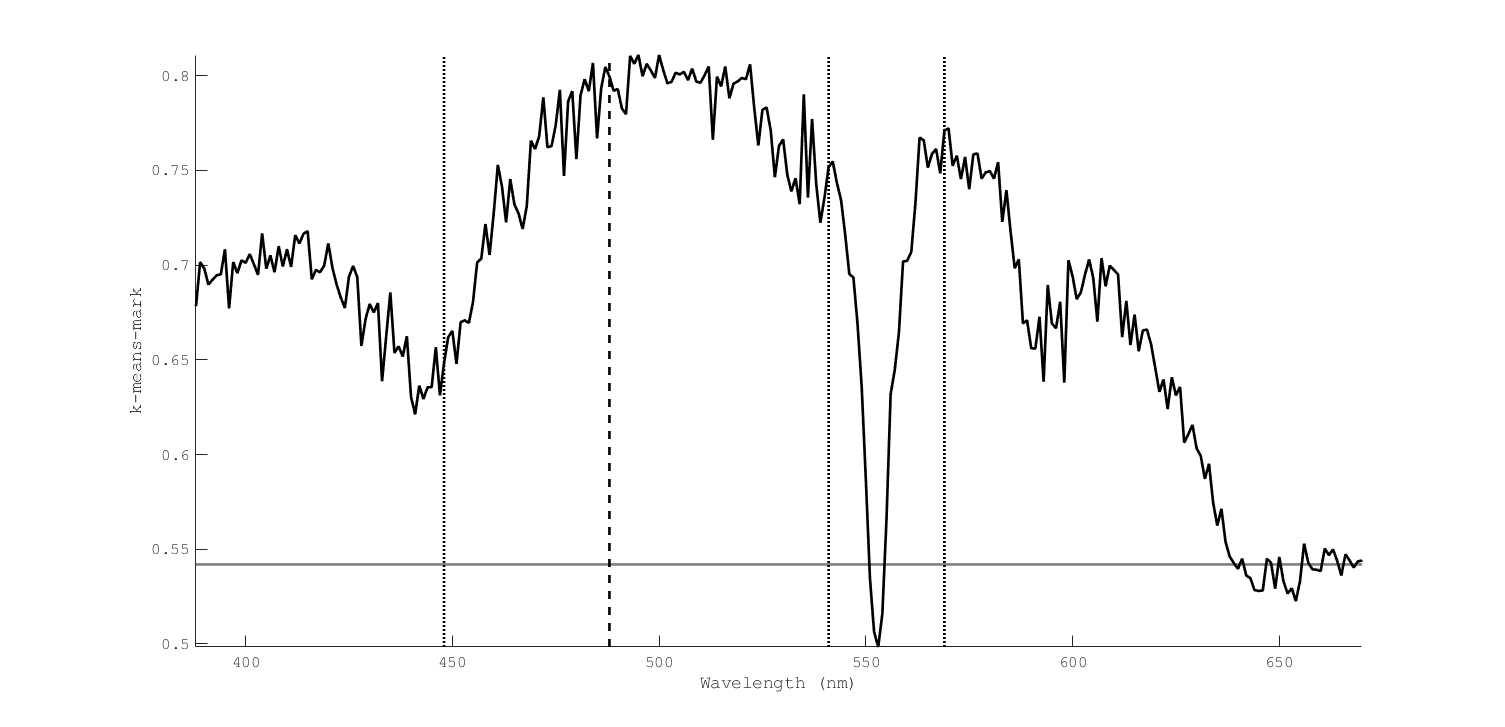
\includegraphics[max width=\textwidth]{figs/comp/melcomp_9/5a_diffMel.png}
 \caption{Testing the effect of shifting the melanopsin sensitivity up and down the spectrum.}
 \label{fig:9opt}
\end{figure} 

% --------------------------------------%

\section{Conclusion}

\subsection{Further work}

\begin{itemize}
\item Further investigate \emph{why} a melanopic transform might work
\begin{itemize}
\item Surface spectral regularities?
\item Test with artificial surfaces and illuminants
\end{itemize}
\item Work out how much of the optimality function is noise
\begin{itemize}
\item Re-run test with random number generators un-set or set with different seeds to understand their influence
\item Consider different observers, daylight data and surface data
\end{itemize}
\item Simplify the grading mechanism (K-means is over the top)
\item Try more complex melanopsin-based transforms
\item Compare and combine with other colour constancy algorithms
\item Don't keep it limited to colorimetry, consider luminance/PC1 also (e.g. \citet{chakrabarti_color_2015}). 
\item Would such a system explain the unexpected results of \citet{cao_evidence_2018}? (LM modulation but not S)
\item If we do use this signal in natural environments, does the degradation of this signal in artificial environments impact our preference ratings? Could evidence of this mechanism show up in lighting preference indices used in the lighting engineering world?
\end{itemize}


% ------------------- %
% EXTRAS



% \begin{figure}[htbp]
%     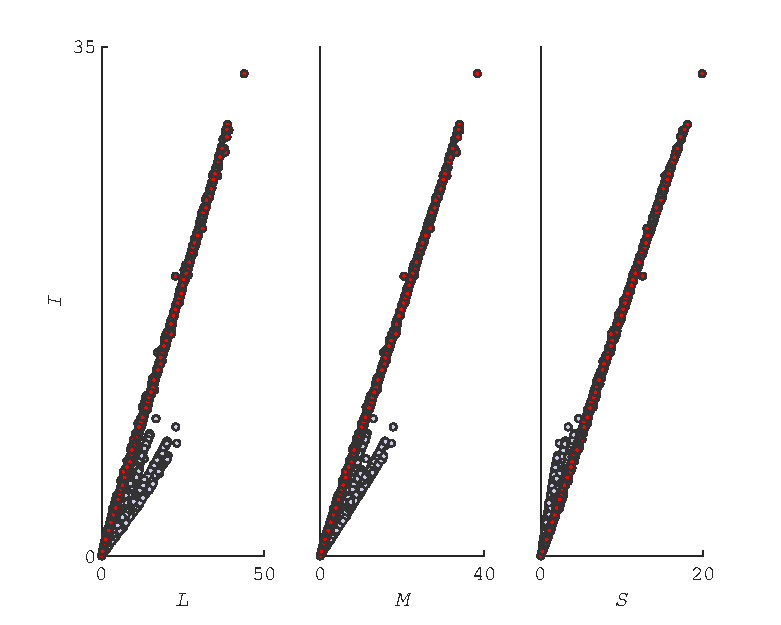
\includegraphics[max width=\textwidth]{figs/comp/melcomp_1/correlationBetweenLevel1Sigs.pdf}
%     \caption{The relationship between melanopic power (analogous to a tristimulus value but calculated using the spectral sensitivity of melanopsin). Red points indicate signals computed directly from the spectral power distribution, grey points represent values of computed colorimetry for objects under illuminants.  The traditional tristimulus values show a very strong correlation for illuminant-only values. It is not particularly easy to see here, but each surface is represented by a roughly straight line of grey points at slightly different angles.}
%     \label{fig:tristimCorrelation}
% \end{figure} 

% It should be noted that there was very high correlation between each signal. This is shown in Figure \ref{fig:tristimCorrelation} and the correlation table below. This can be considered as corresponding to the high importance of the first principal component of the spectral measurements in this dataset. Put another way, a sensor with almost any spectral sensitivity could be used to estimate the general magnitude of the daylight. The discussion of principal components shall be returned to under melcomp\_3.

% \begin{lstlisting}
% corr(LMSI)
%     1.0000    1.0000    0.9993    0.9998
%     1.0000    1.0000    0.9995    0.9999
%     0.9993    0.9995    1.0000    0.9999
%     0.9998    0.9999    0.9999    1.0000
% \end{lstlisting}


